\documentclass[final, 11pt]{article}

\usepackage[italian]{babel}
\usepackage{braket}
\usepackage{diagbox} 
%\usepackage{setspace}
\usepackage{tikz}

\usepackage{amsmath}
\usepackage{amsfonts}
\usepackage{algorithm}		%pseudocodice package
\usepackage{algorithmic}	%pseudocodice package

\usepackage[utf8]{inputenc}

\usepackage{listings}
\usepackage{xcolor}


\usepackage{graphicx}
\usepackage{pdfpages}
\title{Studio di framework per la generazione di fake images di vestiti: Analisi e confronto dei codici VITON e Virtual Try-On with Detail Carving}
\author{ Candidato: Fabio Tarocco VR421748}
\begin{document}
	\clearpage
	
\begin{titlepage}
	\centering
	\vspace*{\fill}
	{\scshape\LARGE Università degli Studi di Verona \par}
	\vspace{1.5cm}
	{\huge Studio di framework per la generazione di fake images di vestiti: Analisi e confronto dei codici VITON e Virtual Try-On with Detail Carving \par}
	\vspace{0.5cm}
	{\scshape  Corso di Laurea Triennale in Informatica \par}
	\vspace{1cm}
	{\Large\itshape Fabio Tarocco VR421748 \par}
	\vspace{1cm}
	\vspace{5cm}
	\vspace*{\fill}
	{\large 16 Ottobre 2020 \par}
\end{titlepage}
	\newpage
	\thispagestyle{plain} % empty
	\mbox{}
	\clearpage
	
	\tableofcontents
	\newpage
	\section{Introduzione al report}
	\subsection{Idea di base}
	La proposta iniziale di stage era quella di analizzare alcuni framework per il riconoscimento dai FAKE images attraverso l’utilizzo di NN e Deep Learning. L’idea era alquanto interessante.
	Per procedere con l’esperienza si è deciso di andare a capire il funzionamento di quello che c’è a monte delle FAKE-IMAGES, cioè la loro creazione.
	
	Si è passati quindi ad un progetto che andasse a studiare il funzionamento e la qualità dei risultati di Frame Work per i virtual Try-On (VTO). La generazione, quindi, di immagini false, artefatte, create attraverso l’utilizzo di codice basato su Reti neurali e Machine Learning, ad hoc per l’ambito della moda e non solo.\\
	Il punto di partenza è stato il codice VITON (portato al CVPR 2018). Una rete per il try-on virtuale image-based (partendo da un dataset di immagini 2D con l’obbiettivo di creare modelli 3D). Codice che sarà la base di partenza e di confronto con gli altri analizzati durante l’esperienza.
	Proseguendo poi al ricercare un concorrente, sempre basato su VITON, per permettere dei confronti prestazionali, nel caso analizzato è stato utilizzato Virtual Try-on with Detail Carving (VTODC). Framework portato al CVPR 2019 e realizzato dalla JDAI CV, con sede a Pechino, che introduce la possibilità di scegliere anche con quale posa generare il modello finale, oltre all’abito e al soggetto.
	
	Infine si è deciso di produrre una demo che permettesse di scegliere una combinazione di soggetti/abiti da un dataset limitato ed eseguire la sostituzione del vestiario con l’opzione di poter introdurre modifiche riguardanti la suddivisione fra i vari segmenti che compongono soggetto di base: vestito, braccia/maniche, pantaloni, viso e capelli.
	
	\subsection {Obiettivi tirocinio}
	L'obbiettivo che ci si è posti come cardine dell'esperienza di tirocinio è stato quello di valutare i risultati, quindi le prestazioni, di più codici che eseguono virtual try-on con base (VITON).
	
	Le richieste erano quelle di capire quando i due codici confrontati producevano output validi e quando invece presentavano difficoltà nel produrli.
	Si è quindi proceduto ad analizzare diversi codici basati sul predecessore VITON e scegliere quelli che potevano avere incrementi sostanziali e visibili nelle prestazioni e nella qualità/affidabilità dei risultati.
	
	Durante l'esperienza si è inoltre deciso di provare ad aggiungere ulteriori obiettivi ossia: Produrre un piccolo applicativo "CANVAS" che permettesse la modifica del label (suddivisione delle componenti del soggetto finale: viso, vestito, braccia, pantaloni, capelli) e applicarlo poi ad una demo "PITON" che permettesse ad un utente di generare differenti outfit, attraverso l'utilizzo di un dataset di campioni ridotto, potendo inoltre utilizzare CANVAS per modificare alcune caratteristiche degli abiti/soggetto.
	
	
	
	\subsection{Cos'è un Virtual Try-On}
	Partiamo spiegando cos'è un virtual try-on. 
	
	È una modalità alternativa con la quale un futuro cliente di un negozio di abbigliamento o di gioielli potrà provare i prodotti dei negozi in modo virtuale, senza dover fisicamente provarli in camerino. Quindi attraverso l'utilizzo di un dispositivo dotato di fotocamera, l'utente può valutare se comprare o meno un capo provandolo virtualmente, attraverso l'utilizzo di realtà aumentata.
	
	Questo approccio, già presente da anni sul mercato ma migliorato mediante l'utilizzo di machine learning
e modelling 3D, permette di provare un capo prima di acquistarlo in qualsiasi luogo, senza l'"obbligo" di andare in negozio, di provare contemporaneamente più capi, valutando anche i vari outfit e soprattutto è time-saving.
	
	Nel caso preso in esame si è operato su codici che prevedevano l'utilizzo di dataset di immagini prese da
un catalogo di abbigliamento di un negozio di e-commerce, quindi non attraverso l'utilizzo di modelling 3D e risultati real-time applicati su video, ma sulla creazione di outfit alternativi a quelli originali utilizzando le coppie modello target e vestito target.
	
	\begin{figure}[!htb]
		\begin{center}
			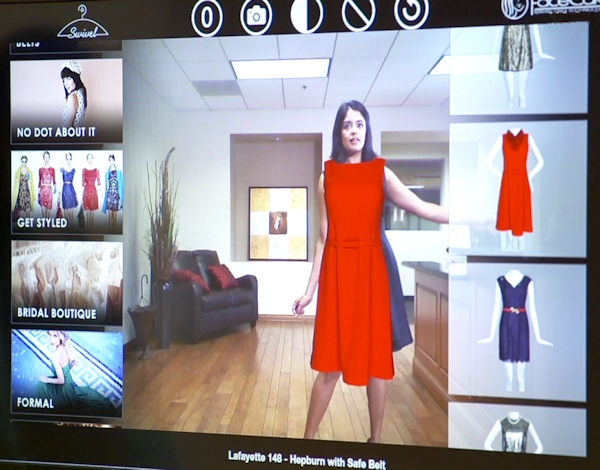
\includegraphics[scale=.7]{FaceCake-virtual-dressing-room.jpg}
		\end{center} \caption{Dressing room dotata di VTO in real time}
	\end{figure} 

	\section{VITON}
	\subsection{Descrizione codice}
	dsad
	\subsection{Qualità output prodotti}	
	L'immagine viene acquisita come una matrice di pixel $ n \times m $, per semplicità assumiamo che essa sia in scala di grigi. Se l'immagine caricata non dovesse essere in \textit{grayScale} è possibile convertirla tramite \texttt{cvtColor( src, src\_gray, COLOR\_BGR2GRAY )}, funzione di \textit{convert color}.
	
	\newpage
	\section{VTO con Detail Carving}
	dsads
	\subsection{Descrizione codice}	
	dsa
	\subsection{Qualità output prodotti}
	Si valutano i segnali che vengono proposti nell'esercizio. Il primo è definito come un segnale con supporto illimitato e con frequenza massima 
	
	\newpage
	\section{Confronto risultati fra i due framework}	
	Si valutano i segnali che vengono proposti nell'esercizio. Il primo è definito come un segnale con supporto illimitato e con frequenza massima 
	
	\newpage
	\section{Variante ACGPN per testing}
	sa
	\subsection{ACGPN in breve}
	dsa
	\subsection{Risultati Demo}
	sa
	
\end{document}